\chapter{Inferência e validação estatística}
\label{chap:validacao}

A precisão da resposta angular e a recuperação dos momentos não bastam
para validar uma inferência. Este capítulo separa a aproximação numérica
da posterior, a adequação da família probabilística e a precisão das
frequências de cobertura estimadas por simulação. A referência A0 conserva
os coeficientes complexos; A e B utilizam as estatísticas do capítulo
anterior. Os controles normais G permitem avaliar o cálculo de A/B sob
experimentos nos quais suas verossimilhanças são exatas.

\section{Parâmetros, prioris e hipóteses comparáveis}

O vetor contínuo de parâmetros é
\begin{equation}
 \theta=(u,g,\gamma,r,t),\quad
 g=\log_{10}A_{\rm gw},\quad
 r=\log_{10}A_{\rm red},\quad t=\log_{10}E.
 \label{eq:inf-parametros}
\end{equation}
Utilizam-se prioris independentes uniformes nessas coordenadas, com
intervalos registrados antes da geração do piloto:
\begin{center}
\begingroup\small\singlespacing
\begin{tabular}{@{}lll@{}}
\toprule
Parâmetro & Suporte & Papel\\
\midrule
\(u=f_gT\) & \([0,1]\) & Dispersão tensorial\\
\(g\) & \([-16,-14]\) & Amplitude do sinal\\
\(\gamma\) & \([3,5{,}5]\) & Inclinação do sinal\\
\(r\) & \([-17,-14{,}5]\) & Amplitude vermelha\\
\(t\) & \([-\log_{10}2,\log_{10}2]\) & Fator branco\\
\bottomrule
\end{tabular}
\endgroup
\end{center}
A inclinação vermelha é fixada em quatro. Os padrões relativos de ruído
dos pulsares são parte do desenho conhecido. Esses intervalos definem
um experimento de validação; não são restrições observacionais derivadas
do TG. A priori uniforme em \(u\) equivale a uma uniforme em massa para
\(T\) fixo. Não equivale a uma uniforme no quadrado ou no logaritmo da
massa, distinção que será examinada na análise de robustez.

O piloto contém 12 direções de Fibonacci, quatro frequências positivas,
\(T=4{,}5\) anos, 118 instantes na grade ideal e distâncias entre 300 e
1000 anos-luz. Permutações independentes fixam a associação das
distâncias, incertezas nominais e padrões vermelhos às direções. Os pesos
de compressão são \(w_n=1/4\). Os 16 vetores iniciais foram sorteados
continuamente da priori, com semente 7070910; os novos dados usam
7070911. Não se sorteiam verdades a partir dos nós de uma quadratura.

A hipótese RG é definida separadamente por \(u=0\), conservando as
mesmas prioris nuisance e a mesma medida de dados. Para qualquer uma
das famílias fixadas, escrevem-se
\begin{align}
 Z_{\rm livre}(y)&=\int_0^1\!du\int
                 L(y\mid u,\eta)\pi(\eta)\,d\eta,\nonumber\\
 Z_{\rm RG}(y)&=\int L(y\mid0,\eta)\pi(\eta)\,d\eta,
 \qquad \eta=(g,\gamma,r,t).
 \label{eq:inf-evidencias}
\end{align}
A probabilidade de massa exatamente nula é zero sob a priori contínua;
ela não representa a probabilidade posterior da hipótese RG. A razão
\(Z_{\rm livre}/Z_{\rm RG}\) só é comparável dentro da mesma medida
de dados. Subtrair log-evidências de A0, A e B entre si não produz um
fator de Bayes entre hipóteses físicas, pois os observáveis e dimensões
mudam. A verificação de evidências é separada da calibração de quantis
\cite{modrak2026bayes}.

\section{Verossimilhanças e normalizações conservadas}

A0 utiliza a normal complexa própria da
Eq.~\eqref{eq:sim-a0}. Há \(M=KN_p=48\) coordenadas complexas,
equivalentes a 96 coordenadas reais. A utiliza quatro vetores reais
de dimensão dez, com a média e a covariância exatas das estatísticas
quadráticas; B utiliza um vetor comprimido de dimensão dez. Em cada
bloco normal,
\begin{equation}
 \log L=-\frac12\left[
 (y-\mu)^T\Sigma^{-1}(y-\mu)+\log\det\Sigma
                         +d\log(2\pi)\right].
 \label{eq:inf-normal}
\end{equation}
O determinante depende dos parâmetros e permanece no cálculo. A mesma
expressão é uma aproximação para os dados físicos A/B e a verossimilhança
exata dos respectivos controles G. As comparações mantêm essa distinção.

As covariâncias são fatoradas por Cholesky. Uma segunda implementação
reutiliza formas quadráticas e coeficientes espectrais entre diferentes
dados, mantendo uma implementação de referência com resoluções diretas.
As verificações independentes confrontam a CN com uma normal real de
dimensão duplicada, a densidade normal com outra implementação e os
momentos polinomiais com traços diretos. A normalização dos dados por
frequência é fixa; não se altera ao variar a amplitude.

\section{Marginalização da escala comum}

Uma redução algébrica torna possível verificar integrais sem depender
apenas da repetição de um amostrador. Definem-se
\(a=g-t\), \(b=r-t\) e \(s=10^t\). A transformação inversa
tem Jacobiano unitário nas coordenadas logarítmicas. Se \(G,R,E\)
denotam os intervalos originais de \(g,r,t\), os limites condicionais
da escala são
\begin{align}
 t_-&=\max(E_-,G_--a,R_--b),\nonumber\\
 t_+&=\min(E_+,G_+-a,R_+-b).
 \label{eq:inf-suporte-escala}
\end{align}
Somente pontos com \(t_+>t_-\) pertencem ao suporte. A densidade
induzida das razões é
\begin{equation}
 \pi(a,b)=\frac{t_+-t_-}{\Delta G\,\Delta R\,\Delta E},
 \qquad \operatorname{Cov}(a,b)=\operatorname{Var}(t).
 \label{eq:inf-prior-razoes}
\end{equation}
Logo, duas prioris uniformes independentes nas razões mudariam o modelo.
Uma transformação de Rosenblatt condicional amostra exatamente essa
densidade. Nesse caso, integra-se a média condicional
\(\int_{t_-}^{t_+}L\,dt/(t_+-t_-)\). Na cubatura direta em
\((a,b,\gamma)\), utiliza-se a integral sem esse divisor, multiplicada
pela densidade da caixa original. São duas representações da mesma
medida, que não podem ser combinadas contando o volume duas vezes.

Todas as parcelas de covariância recebem a escala comum:
\(C_n(t)=s^2C_{0n}\). Para A0, definem-se
\begin{equation}
 \chi=\sum_nq_n^\dagger C_{0n}^{-1}q_n,\qquad
 D_C=\sum_n\log\det C_{0n}.
 \label{eq:inf-chi-cn}
\end{equation}
Com \(v=\chi10^{-2t}\), a integral normalizada em escala é
\begin{equation}
 I_{\rm CN}=\frac{\pi^{-M}e^{-D_C}\chi^{-M}}{2\ln10}
 \int_{\chi10^{-2t_+}}^{\chi10^{-2t_-}}
           v^{M-1}e^{-v}\,dv.
 \label{eq:inf-escala-cn}
\end{equation}
O caso \(\chi=0\) tem limite exponencial elementar. Diferenças de
gamas incompletas, séries positivas e a forma finita da cauda superior
para \(M\) inteiro evitam perder a integral por subfluxo antes de
tomar seu logaritmo.

Para a família normal, \(\mu=s^2\mu_0\) e
\(\Sigma=s^4\Sigma_0\). Somando os blocos, sejam
\begin{align}
 X&=y^T\Sigma_0^{-1}y,&
 B&=\mu_0^T\Sigma_0^{-1}y,\nonumber\\
 C&=\mu_0^T\Sigma_0^{-1}\mu_0,&
 D_\Sigma&=\log\det\Sigma_0.
 \label{eq:inf-coeficientes-normal}
\end{align}
Aqui \(B\) é um coeficiente escalar, sem relação com o nome da análise
comprimida. Com \(z=10^{-2t}\), resulta
\begin{equation}
 I_{\mathcal N}=
 \frac{e^{-[D_\Sigma+C+d\log(2\pi)]/2}}{2\ln10}
 \int_{10^{-2t_+}}^{10^{-2t_-}}
        z^{d-1}e^{-Xz^2/2+Bz}\,dz.
 \label{eq:inf-escala-normal}
\end{equation}
A potência é \(d-1\), pois a medida contribui com \(dz/z\).
As dimensões reais são 40 para A e dez para B. O log-integrando é
côncavo em \(z>0\); limites por tangentes controlam as caudas
descartadas e duas ordens de Gauss--Legendre verificam a parte retida.
Ordens ou orçamentos insuficientes produzem falha explícita.

As CDFs da escala são razões das mesmas integrais truncadas.
As amplitudes originais usam os limites \(x-a\) e \(x-b\).
Uma alternativa integra uma caixa original truncada em cada limiar,
com o fator de volume correspondente. Ela alinha os painéis às mudanças
dos limites condicionais, evitando que uma integral de evidência
convergida seja tomada por prova de convergência dos quantis.

Na reprodução integrada, 90 integrais CN concordaram com quadratura
direta em \(t\) até \(8{,}18\times10^{-10}\) no logaritmo;
42 CDFs concordaram até \(1{,}42\times10^{-14}\).
Para a família normal, 162 casos cobriram sinais diferentes do termo
linear, intervalos estreitos e caudas. Acima de logdensidade
\(-10^5\), a maior diferença foi \(2{,}92\times10^{-11}\).
Caudas extremas foram confrontadas com integração de 70 dígitos,
com erro absoluto máximo de \(2{,}98\times10^{-7}\) em
logdensidades próximas de \(-5\times10^8\). Essa limitação de
ponto flutuante é registrada separadamente da tolerância de quadratura.
As nove comparações com a verossimilhança física original, integrada
diretamente em escala, concordaram até \(3{,}20\times10^{-10}\).
Esses resultados verificam a redução condicional; a integração externa
e a calibração da inferência exigem controles próprios.

\section{Referência independente em uma realização}

A realização de índice 14 do piloto foi escolhida como referência
determinística de A0. A decomposição espectral da matriz angular
branqueada pelo ruído permite reutilizar autovalores ao variar a
amplitude e a inclinação do sinal. O cálculo preserva os autovalores
e verifica a positividade dos denominadores espectrais. Em 972
comparações com Cholesky, a diferença máxima de log-verossimilhança
foi \(3{,}37\times10^{-11}\).

A Fig.~\ref{fig:inf-cubatura} ilustra uma distinção da validação.
A evidência da primeira rota converge ao refinar a ordem, mas algumas
CDFs não satisfazem a tolerância. Os cortes adicionais das CDFs
precisam entrar na partição dos painéis. Com caixas truncadas
alinhadas a esses cortes, a comparação entre ordens \(20^3\) e
\(32\times20\times12\) reduziu a maior diferença de CDF, nos vinte
cortes previamente congelados, de \(4{,}65\times10^{-3}\) para
\(1{,}18\times10^{-4}\). Nesse alvo, o refinamento independente
da malha de massa de 75 para 139 nós produziu diferença de
\(1{,}96\times10^{-5}\) em \(\log Z\), sem interpolar matrizes
entre os nós durante a cubatura.

\begin{figure}[htbp]
 \centering
 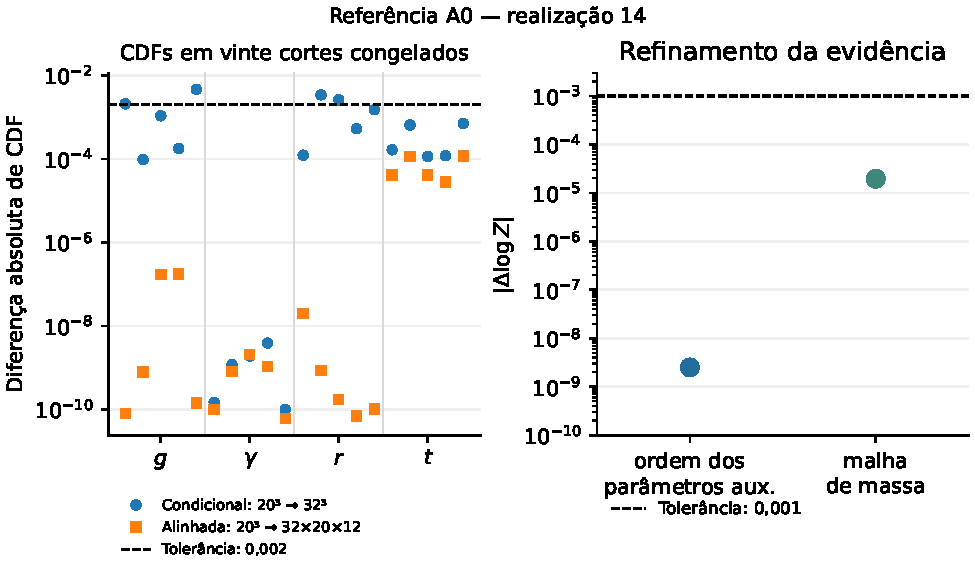
\includegraphics[width=\textwidth]{../figures/C07/cubatura_convergencia.pdf}
 \caption{Verificações separadas da cubatura de A0 na realização 14.
 À esquerda, cada parâmetro auxiliar tem quatro cortes de quantis
 preliminares e um corte na verdade, mantidos fixos durante a comparação.
 À direita, a convergência da evidência não diagnostica sozinha as CDFs.
 As linhas indicam as tolerâncias previamente definidas.
 Esta figura não representa a campanha SBC.}
 \label{fig:inf-cubatura}
\end{figure}

A localização final usa intervalos comuns às quatro combinações de
ordem e malha. Os dezesseis intervalos de quantis auxiliares tiveram
largura \(0{,}0009\) da largura da priori. Seu ponto médio fica a
no máximo \(0{,}00045\) dessa largura do quantil de cada CDF numérica
comparada. A Tabela~\ref{tab:inf-quantis-ref} registra os pontos médios.
Os arquivos conservam extremos, CDFs e diferenças entre resoluções.
O maior limite explícito de contribuições dispensadas, no controle
por quadratura sem omissão, foi \(1{,}30\times10^{-14}\).
Esse limite controla a omissão de nós da regra finita; não é um
limite analítico do erro da integral contínua.

\begin{table}[htbp]
 \centering\small\singlespacing
 \caption{Quantis de referência de A0, realização 14, nas coordenadas
 da Eq.~\eqref{eq:inf-parametros}. A precisão é descrita pelos
 intervalos comuns de refinamento.}
 \label{tab:inf-quantis-ref}
 \begin{tabular}{@{}lrrrr@{}}
 \toprule
 Parâmetro & \(Q_{05}\) & \(Q_{50}\) & \(Q_{90}\) & \(Q_{95}\)\\
 \midrule
 \(u\)      & 0,05693 & 0,53874 & 0,91332 & 0,95697\\
 \(g\)      & -15,9104 & -15,1627 & -14,6415 & -14,5509\\
 \(\gamma\) & 3,1366 & 4,2502 & 5,2125 & 5,3519\\
 \(r\)      & -14,9808 & -14,5966 & -14,5258 & -14,5142\\
 \(t\)      & -0,2981 & -0,2679 & -0,2159 & -0,1984\\
 \bottomrule
 \end{tabular}
\end{table}

Uma pequena largura horizontal não garante erro vertical igualmente
pequeno: o envelope de \(F(q_{\mathrm{mid}})-p\), obtido por
monotonicidade, alcança \(0{,}00607\) em um intervalo. A CDF não
foi calculada diretamente em cada ponto médio. A comparação com
amostras posteriores usa, portanto, desigualdades nos extremos,
sem substituir automaticamente \(F(q_{\mathrm{mid}})\) por \(p\).
A implementação portada reproduziu exatamente a evidência condicional
e as vinte CDFs de controle em \(u=0{,}5\).

Nesta realização, a cubatura fina deu
\(\log Z_{\rm livre}\simeq-76{,}0801\) e
\(\log(Z_{\rm livre}/Z_{\rm RG})\simeq0{,}1320\).
São resultados de um único dado sintético, dentro da mesma família CN
e medida amostral. Essa referência não aprova automaticamente outros
alvos, a interpolação angular ou uma campanha de calibração.

\section{Diagnósticos que dependem dos dados}

Na SBC, a verdade é sorteada da priori e os dados são sorteados
condicionalmente à verdade \cite{talts2018}. Além de
\(F_j(\theta_j^{\rm verdadeiro}\mid y)\), considera-se
\begin{equation}
 U_L=\Pr_{\theta\mid y}
  \left[\log L(y\mid\theta)\leq
        \log L(y\mid\theta^{\rm verdadeiro})\right].
 \label{eq:inf-pit-logl}
\end{equation}
A quantidade utiliza o mesmo dado e a mesma família probabilística,
incluindo seus determinantes. Um algoritmo que sempre devolve a priori
pode passar nos postos marginais dos parâmetros. Quantidades dependentes
do dado tornam o diagnóstico sensível a outras falhas
\cite{modrak2025}. SBC global tampouco garante precisão em toda região
ou para toda realização \cite{sailynoja2026}.

Os utilitários foram verificados primeiro em um modelo normal--normal
conjugado, sem significado físico de PTA, com cinco coordenadas,
4096 realizações e um prefixo de 500 definido antecipadamente. A
posterior analítica não apresentou rejeições na família de 31 testes
com correção de Holm. O controle que ignora os dados passou nos PITs
dos parâmetros, mas falhou fortemente na quantidade da
Eq.~\eqref{eq:inf-pit-logl}, com estatística KS aproximadamente
\(0{,}974\). Uma rejeição adicional de cobertura nominal do controle
negativo foi preservada como flutuação do experimento; sementes e
limiares não foram escolhidos após os resultados. Esse exemplo valida
o diagnóstico, sem constituir uma SBC da inferência de PTA.

Para 500 realizações independentes e cobertura populacional de 90\%,
o erro-padrão binomial é
\(\sqrt{0{,}9(1-0{,}9)/500}=0{,}0134\).
Contagens e intervalos binomiais exatos acompanham a fração estimada.
Contrastes entre análises da mesma realização usam diferenças pareadas.
O protocolo científico fixa 31 hipóteses por análise: seis PITs, vinte
coberturas unilaterais nos níveis 0,05, 0,50, 0,90 e 0,95, e cinco
coberturas centrais de 90\%. Aplicam-se correções de Holm em famílias
separadas: 93 hipóteses para A0\_CN/A\_G/B\_G e 62 para A\_CN/B\_CN.
Os quinze contrastes pareados de cobertura central usam o teste exato
de McNemar, com sua própria correção de Holm. Não se reivindica controle
global de 5\% ao reunir conclusões dessas famílias diferentes.

Em injeções fixas, não se exige uniformidade universal dos PITs ou
cobertura frequentista nominal dos intervalos bayesianos. Em particular,
\([0,U_{90}]\) cobre \(u=0\) estruturalmente em 100\% dos casos
admissíveis, enquanto um intervalo contínuo de caudas iguais pode
excluir a fronteira. Ausência de sinal e sinal com massa nula são
experimentos diferentes; amplitude exatamente zero está fora do suporte
de uma priori logarítmica finita.

\section{Erro Monte Carlo da posterior}

O protocolo de cadeias separa mistura, precisão e erro determinístico.
Quatro cadeias conservam sua ordem temporal; o aquecimento é descartado
e a proposta permanece fixa na produção. Nas coordenadas
\(x_j=(\theta_j-a_j)/(b_j-a_j)\) e \(z_j=\operatorname{logit}(x_j)\),
a densidade alvo da priori uniforme deve incluir
\begin{equation}
 \log p(z\mid y)=\log L(y\mid\theta(z))+
       \sum_j[\log x_j+\log(1-x_j)]+\text{constante}.
 \label{eq:inf-jacobiano-logit}
\end{equation}
A log-verossimilhança é armazenada separadamente desse Jacobiano para
a Eq.~\eqref{eq:inf-pit-logl}. Sementes, ordem dos alvos, proposta,
tabela angular e duração identificam cada execução.

Utilizam-se \(\widehat R\) com divisão das cadeias, normalização de
postos e dobramento em torno da mediana, além de tamanhos efetivos
para a região central e as caudas \cite{vehtari2021}. Exigem-se
\(\widehat R\leq1{,}01\) e tamanhos efetivos pelo menos 400,
incluindo a log-verossimilhança. Esses pisos não garantem a precisão
necessária de uma CDF. Para cada um dos vinte cortes marginais,
das cinco verdades e da log-verossimilhança verdadeira, o protocolo
registra o erro da média do indicador correspondente. Conserva-se o
maior erro estimado por autocorrelação e por médias de lotes.
No protocolo inicial, cada cadeia utiliza lotes de comprimento
\(\lceil\sqrt{N}\rceil\), pelo menos dezesseis lotes completos,
e comprimento pelo menos cinco vezes o tempo de autocorrelação
estimado. Uma regra insuficiente produz falha documentada.

A meta é erro-padrão Monte Carlo de CDF no máximo \(0{,}00335\).
Em uma CDF próxima de \(1/2\), isso requer aproximadamente
22\,277 amostras efetivas do indicador. Um indicador constante por
falta de visitas a uma cauda não recebe erro artificialmente nulo.
Exceções estruturais conhecidas, como \(F_u(0)=0\), são identificadas
separadamente. A comparação com o intervalo de referência
\([\ell_p,h_p]\) utiliza
\begin{align}
 \widehat F_{\rm MC}(\ell_p)&\leq p+\epsilon_{\rm det}
       +z_{1-0{,}05/40}\,\operatorname{MCSE}[\widehat F_{\rm MC}(\ell_p)],\nonumber\\
 \widehat F_{\rm MC}(h_p)&\geq p-\epsilon_{\rm det}
       -z_{1-0{,}05/40}\,\operatorname{MCSE}[\widehat F_{\rm MC}(h_p)].
 \label{eq:inf-referencia-mcmc}
\end{align}
São quarenta desigualdades unilaterais para vinte quantis, com a mesma
correção de Bonferroni de vinte comparações bilaterais e erro
determinístico expresso na unidade de CDF. Exige-se também a meta de
MCSE em ambos os extremos. Uma tolerância horizontal de quantil não
pode ser somada diretamente a essa probabilidade. Cadeias Metropolis
não fornecem a evidência marginal como subproduto.

Os diagnósticos foram verificados em processos normais independentes
e autorregressivos de primeira ordem. Para correlação \(0{,}8\), o
tamanho efetivo estimado da média foi 93,8\% do valor teórico; para
o indicador em zero, foi 96,2\%. Em 128 repetições, a dispersão
empírica da CDF dividida pelo erro estimado foi 1,12. Esses controles
avaliam a estimativa de erro, sem simular uma PTA.

Uma segunda verificação mostra por que adicionar um sorteio uniforme
a postos discretos não elimina a dependência entre amostras.
Em 2048 experiências com 64 amostras posteriores normais, os postos
aleatorizados independentes tiveram \(D_{\rm KS}=0{,}0116\).
Com as mesmas marginais corretas, mas correlação autorregressiva
\(0{,}95\), obteve-se \(D_{\rm KS}=0{,}1325\).
Intercambiabilidade com a verdade não decorre da distribuição marginal
correta, nem de substituir o número de passos pelo tamanho efetivo.
Na campanha, o KS contínuo ideal recebe uma análise de sensibilidade
aos erros dos PITs; não é apresentado como teste finito exato de
uma CDF MCMC aproximada.

\section{Integração com sorteios independentes}

Uma alternativa ao uso direto das cadeias é ajustar uma proposta conjunta
\(q_z\) durante um piloto e congelá-la antes de novos sorteios independentes.
Nas coordenadas da Eq.~\eqref{eq:inf-jacobiano-logit}, os pesos completos são
\begin{equation}
 \log w_i=\log L(y\mid\theta(z_i))+
       \sum_j[\log x_{ij}+\log(1-x_{ij})]-\log q_z(z_i).
 \label{eq:inf-peso-iid}
\end{equation}
O volume da caixa da priori cancela com a parte afim do Jacobiano.
A densidade avaliada é a da mistura inteira, incluindo todas as
probabilidades dos componentes. A componente defensiva melhora o suporte
prático; sua presença não certifica a exploração de todos os modos.

Para um indicador \(h_i=\mathbf1\{g(\theta_i)\leq c\}\), sejam
\(p_i=w_i/\sum_jw_j\) e \(\widehat F=\sum_i p_i h_i\). A expansão delta
para a razão das médias fornece a variável de influência
\begin{equation}
 \psi_i=Np_i(h_i-\widehat F),\qquad
 \widehat{\operatorname{MCSE}}_{\rm IID}^2
       =\frac{\operatorname{Var}_{\rm amostral}(\psi_i)}{N}.
 \label{eq:inf-iid-influencia}
\end{equation}
Ela conserva a covariância entre numerador e denominador; não transforma
pesos em contagens binomiais. A variância usa correção \(N-1\).
A expressão concorda com a forma auto-normalizada discutida por
\textcite{vehtari2024psis}. Os pesos aqui são brutos: não se implementou
suavização Pareto e não se reivindicam seus diagnósticos de cauda.

Em quatro replicações de mesmo tamanho e mesma proposta congelada,
calcula-se também a dispersão das influências de bloco
\((\widehat Z_r/\widehat Z)(\widehat F_r-\widehat F)\).
Adota-se o maior erro entre essa estimativa e a Eq.~\eqref{eq:inf-iid-influencia}.
A estimativa entre quatro blocos é instável e constitui um controle
adicional, sem garantia finita de cobertura. Registram-se concentração
dos pesos, peso máximo, subfluxos numéricos e indicadores constantes.
Uma guarda de dominância exige
\(p_{\max}/(1-p_{\max})\leq0{,}00335\); ela limita o efeito observado
da exclusão de um ponto, sem limitar massa posterior não visitada.

O controle conjugado normal--normal executou 128 campanhas com quatro
replicações em cada um dos tamanhos 1024 e 8192. Há solução analítica para
CDFs marginais, evidência e CDF de log-verossimilhança. As razões entre
dispersão empírica e MCSE de influência ficaram entre 0,935 e 1,037;
o refinamento reduziu a MCSE por fatores entre 0,353 e 0,354.
Os sete critérios prospectivos passaram na reexecução integrada.
Um controle com modo raro não visitado foi sinalizado em todas as
campanhas, embora o ESS de pesos pudesse parecer elevado. Esse resultado
expõe uma falha possível; não demonstra que as mesmas guardas detectem
todo modo ausente em uma PTA.

A uniformidade SBC requer cinco PITs marginais e o PIT da
Eq.~\eqref{eq:inf-pit-logl}; os vinte cortes nos quantis têm finalidade
adicional de descrever limites e intervalos. O tamanho da produção deve
ser fixado por pilotos independentes, sem usar as verdades das novas
simulações para ajustar a proposta ou decidir quais realizações conservar.
A evidência pode ser registrada como diagnóstico de normalização, mas
sua utilização científica exige precisão e comparação sob a mesma
medida de dados. Nenhum fator de Bayes entre espaços A0/A/B é definido.

Para distinguir a variabilidade entre realizações do erro de integração,
o protocolo acrescenta um envelope de sensibilidade. Para cada uma das
15\,000 CDFs de verdade, sejam
\begin{equation}
 \begin{aligned}
 [L_i,U_i]&=[0,1]\cap
 \left[\widehat F_i-\delta_i,\widehat F_i+\delta_i\right],\\
 \delta_i&=0{,}002+z_{\rm MC}\,\widehat{\operatorname{MCSE}}_i,
 \qquad z_{\rm MC}=\Phi^{-1}\!\left(1-\frac{0{,}01}{2\times15\,000}\right).
 \end{aligned}
 \label{eq:inf-pit-envelope}
\end{equation}
Essa construção é assintótica. O termo 0,002 representa a escala de
sensibilidade numérica fixada, sem constituir uma cota analítica uniforme.
Uma função não resolvida recebe \([L_i,U_i]=[0,1]\); a realização permanece
no denominador. Resolução exige sua precisão, seus contrastes entre
replicações e níveis, além das guardas comuns de pesos e normalização.
A falha de outro PIT é registrada separadamente. Os vinte cortes
adicionais continuam necessários para os produtos de quantis a que
se referem, sem se tornarem vinte novos PITs de SBC.

Condicionalmente à validade dos intervalos, a CDF empírica ideal fica
entre
\begin{equation}
 G_-(v)=\frac1{500}\sum_i\mathbf1\{U_i\leq v\},\qquad
 G_+(v)=\frac1{500}\sum_i\mathbf1\{L_i\leq v\}.
 \label{eq:inf-ecdf-envelope}
\end{equation}
Essas curvas são distintas de uma banda amostral de uniformidade entre
as 500 realizações. Contagens certamente e possivelmente cobertas
propagam a mesma incerteza para intervalos e testes binomiais. Limites
conservadores para as estatísticas KS e os valores de \(p\) mostram se
uma decisão de Holm resiste à variação numérica permitida. Uma ausência
de rejeição, especialmente com funções não resolvidas, não certifica
calibração ou equivalência entre análises.

\section{Validação da interpolação e do piloto}

A dependência angular contém fases oscilatórias dos pulsares. Verificar
\(\Gamma\) em alguns nós não permite interpolar arbitrariamente entre eles.
A tabela final utiliza 8336 nós e uma cúbica na coordenada
\(-\beta_1=-\sqrt{(1-u)(1+u)}\). A integral tensorial isotrópica é par em
\(\beta_1\): a mudança \(\Omega\mapsto-\Omega\) troca seu sinal, enquanto
as demais \(\beta_n\) dependem de \(\beta_1^2\). Por isso a derivada no
extremo \(\beta_1=0\) é nula. Impõe-se essa condição; no outro extremo,
usa-se a condição \textit{not-a-knot}. A priori permanece uniforme em \(u\).

Os quatro controles de Bernstein de cada trecho cúbico são matrizes
hermitianas. Quando todos são positivos semidefinidos, sua combinação
com os polinômios de Bernstein preserva essa propriedade no intervalo.
Na tabela final, o menor autovalor calculado foi aproximadamente
\(-2{,}8\times10^{-16}\), dentro da tolerância numérica de \(10^{-12}\).
Não houve trechos substituídos por interpolação linear, recorte de
autovalores ou adição de ruído artificial. As médias e covariâncias
inferenciais são reconstruídas da mesma matriz interpolada; a covariância
das estatísticas é quadrática em seus componentes, não uma interpolação
independente dos valores de covariância nos extremos.

As primeiras tabelas falharam, inclusive uma malha uniforme de 8193 pontos
na coordenada \(\beta_1\). O erro de verossimilhança concentrava-se perto
da fronteira cinemática, onde uma pequena perturbação angular pode ser
relevante para a fatoração. O refinamento acrescentou 142 nós locais e
foi seguido por novos pontos independentes. A Tabela~\ref{tab:inf-orf}
registra o confronto final, mantendo a tolerância prospectiva
\(10^{-3}\) em log-verossimilhança. Trata-se de validação no conjunto
explicitado, sem prova analítica de erro uniforme em toda a caixa.

\begin{table}[htbp]
\centering
\caption{Verificação final da tabela angular de inferência, no experimento de 12 pulsares e 4 frequências.}
\label{tab:inf-orf}
\begin{tabular}{lrr}
\toprule
Conjunto de confronto & Avaliações & Maior \(\lvert\Delta\log L\rvert\)\\
\midrule
Pontos posteriores, 4169--8336 nós & 82\,240 & \(4{,}93\times10^{-6}\)\\
Nova amostra da priori & 4\,096 & \(8{,}82\times10^{-4}\)\\
Novos nós do refinamento & 333\,360 & \(2{,}10\times10^{-4}\)\\
144 massas independentes, malhas & 11\,520 & \(1{,}95\times10^{-5}\)\\
Mesmas massas, tabela fina--ORF direta & 11\,520 & \(2{,}57\times10^{-7}\)\\
500 verdades novas, cinco análises & 2\,500 & \(1{,}85\times10^{-8}\)\\
\bottomrule
\end{tabular}
\end{table}

O piloto inferencial subsequente reteve dezesseis alvos selecionados
entre os oitenta pares de realização e análise dos testes de engenharia.
A proposta em cinco logits combina quatro normais e uma componente
Student defensiva, com parâmetros ajustados previamente e congelados.
Uma auditoria confrontou densidades, sorteios e normalização da proposta
com cálculos independentes. O número de sorteios foi planejado por uma
grade de CDFs dos parâmetros e de log-verossimilhança em pilotos distintos,
sem consultar as verdades para determinar esse tamanho.

Executaram-se dois níveis novos de 16\,384 e 65\,536 sorteios por
replicação, com quatro replicações cada. O nível maior satisfez a meta
nos 416 cortes de CDF e a guarda de pesos nos dezesseis alvos; a maior
MCSE foi \(0{,}002985\). Os vinte brackets de A0 na realização 14
satisfizeram simultaneamente a precisão dos extremos e a comparação
com cubatura. Não houve discordância nos 3264 contrastes entre
replicações nem nos 152 contrastes de refinamento das famílias
prospectivas. No nível menor, apenas 385 dos 416 cortes passaram.
Essas contagens se referem a funções e alvos do piloto, não a
416 realizações independentes de uma PTA.

Os protocolos e resultados reprovados permanecem preservados. O
piloto aprovado não autoriza presumir precisão em qualquer dado futuro:
o ajuste da proposta por realização e os erros de cada função precisam
acompanhar a campanha. Os dezesseis dados de engenharia são excluídos
do denominador da SBC de produção.

Um segundo ensaio integrou o fluxo completo a partir de propostas
treinadas a frio, com 8192 passos por cadeia, quatro cadeias e 2048
estados para ajustar a mistura. Ele satisfez os vinte brackets de A0,
mas apenas 401 das 416 CDFs atingiram a precisão requerida. No alvo
A\_CN associado ao dado d9, o maior peso normalizado foi cerca de
1,13\% e a maior MCSE, 0,0125. Esse caso reprovou a guarda de dominância.
O ensaio distingue o cálculo correto dos pesos da adequação de uma
proposta aprendida em uma execução particular. A falha permanece no
registro de engenharia; o piloto com propostas previamente aquecidas
não a substitui.

A reprodução desse alvo recuperou exatamente os oito arquivos brutos
originais. A densidade da proposta foi confrontada com distribuições
SciPy independentes, e os vinte maiores pesos receberam uma avaliação
direta por Cholesky. Os maiores desvios em logaritmo foram
\(1{,}64\times10^{-13}\) e \(2{,}85\times10^{-14}\), respectivamente.
O ponto de maior peso estava próximo ao limite superior da priori de
amplitude gravitacional, em uma região pouco coberta pelas quatro
Gaussianas ajustadas. Aumentar o treino não resolveu sistematicamente
essa deficiência local: propostas de sementes diferentes podiam aumentar
ou diminuir a densidade naquela região.

Foi então fixada, antes da produção principal, a transformação
\begin{equation}
 q_{\mathrm{ampla}}(z)=0{,}75\,G(z;C)
       +0{,}10\,G(z;9C)+0{,}15\,t_5(z),
 \label{eq:proposta-ampla}
\end{equation}
em que \(G\) denota a mistura de quatro componentes já ajustada.
As quatro médias e seus pesos relativos são repetidos na parte ampla;
a Student global, incluindo sua escala, permanece a mesma. Não há um
novo ajuste nem uso da verdade injetada. Como
\(q_{\mathrm{ampla}}\geq(15/17)q_{\mathrm{original}}\), a nova proposta
preserva um limite inferior pontual em todo o espaço logit. Para uma CDF
com variância assintótica de importância finita, segue
\(V_{\mathrm{ampla}}\leq(17/15)V_{\mathrm{original}}\).
Essa desigualdade limita uma possível piora assintótica; não garante
que uma produção finita satisfaça a meta de erro.

Uma produção independente com as dezesseis propostas transformadas
satisfez 416 de 416 CDFs, os 96 PITs, as dezesseis guardas de peso e os
vinte brackets de referência no nível \(65536\times4\).
A maior MCSE foi \(0{,}002624\). Não houve discordância ou erro não
resolvido nos 3264 contrastes entre réplicas e nos 152 de refinamento.
Uma grade adicional de 54 cortes por alvo, fixada sem as verdades,
passou nos 864 cortes e foi reproduzida por um leitor independente.
O nível menor conservou suas falhas: apenas 375 de 416 CDFs satisfizeram
a precisão formal. Os dois níveis continuam necessários para avaliar
refinamento, sem interpretar o nível menor como posterior aprovada.

A implementação integrada preserva o ajuste original e calcula uma
nova identidade da proposta depois da transformação. Um teste adicional
do fluxo completo, em três alvos de engenharia, verificou essas
identidades, os diagnósticos e o arquivo reprodutível. A regra
\eqref{eq:proposta-ampla} foi congelada para todos os alvos da campanha;
casos numericamente não resolvidos permanecem no inventário.

\section{Geração independente da campanha}

Foram geradas 500 verdades novas da priori, com semente 707409101,
e observações com semente 707409102. Cada massa verdadeira é contínua;
não se escolhe entre os nós da interpolação. O gerador calcula e verifica
a ORF diretamente nessa massa, antes de gerar a observação física e o
controle gaussiano pareado. Incluindo as âncoras, foram preservados
503 nós, com refinamento angular e sete confrontos independentes.
O maior desvio entre as resoluções angulares foi
\(8{,}18\times10^{-13}\); nos confrontos diretos, foi
\(4{,}75\times10^{-15}\). Todos os dados foram regenerados e comparados
com tolerância \(10^{-12}\), a partir de configurações e fontes com
hashes registrados.

Uma reconstrução independente, sem chamar as rotinas de covariância
e geração pareada do integrador, refez os 500 sorteios e os produtos de
pares. Os maiores desvios, em unidades dos desvios-padrão pertinentes,
foram \(7{,}4\times10^{-16}\) para os coeficientes complexos,
\(4{,}5\times10^{-15}\) para as estatísticas quadráticas e
\(2{,}94\times10^{-15}\) para o controle normal. Nos extremos de sinal
e condicionamento da amostra, uma representação real independente
recuperou os momentos de Isserlis. Separadamente, a verossimilhança
interpolada foi comparada com as ORFs diretas nas 500 verdades e cinco
análises: o maior desvio foi \(1{,}85\times10^{-8}\). Esse confronto
amplia o conjunto validado, sem ser uma prova uniforme para toda posterior.

Também foram geradas 32 observações por cenário fixo: sinal com \(u=0\),
sinal próximo ao limiar com \(u=0{,}995\) e ausência de sinal
gravitacional. As duas massas definidas receberam ORFs diretas próprias;
no terceiro cenário, a contribuição gravitacional foi exatamente zero.
Nesse caso, massa, amplitude e inclinação gravitacionais não têm uma
verdade finita a recuperar. Suas máscaras impedem calcular PITs ou
coberturas fictícias. Os 96 dados foram reproduzidos bit a bit. Essa
amostra menor fornece um diagnóstico condicional: a 90\% de cobertura,
seu erro-padrão populacional seria 5,3 pontos percentuais, distinto dos
1,34 pontos da campanha de 500.

\section{Calibração das 500 realizações}
\label{sec:c07-resultados-sbc}

A campanha concluiu as cinco análises de cada uma das 500 realizações,
sem substituir dados ou sementes depois de observar os diagnósticos.
O treino usou a semente 907110101; a produção, 907110102, com quatro
réplicas independentes nos níveis 16384 e 65536. Foram contabilizadas
81930000 avaliações de verossimilhança no treino, incluindo a
inicialização, e 819200000 na produção: 901130000 no total.
Os registros de todas as 2500 inferências foram arquivados antes de
retirar os arquivos brutos regeneráveis. A conclusão de um arquivo
não implica aprovação dos seus diagnósticos.

Em 81 inferências, ao menos um dos cinco controles agregados de
precisão, pesos, réplicas, refinamento e referência não foi satisfeito.
Essa contagem inclui os vinte cortes adicionais selecionados no nível
menor e não coincide com a resolução de cada PIT. Aplicando a regra
por função, 243 dos 15000 PITs ficaram numericamente não resolvidos;
seus envelopes foram mantidos como \([0,1]\). Os 500 dados de cada
modelo participam de todos os testes e coberturas. Não se calculou
uma SBC apenas sobre os casos aprovados.

As tabelas seguintes distinguem contagens de funções resolvidas,
testes nominais e sensibilidade numérica. Os envelopes incorporam
\(0{,}002+4{,}97083\,\mathrm{MCSE}\) para as funções resolvidas,
conforme o protocolo prospectivo. Sua validade continua condicional
à aproximação assintótica de Monte Carlo e à margem operacional de
refinamento; não se convertem em uma garantia global da integral.

% Automatically rendered from a complete C07 summary; no new statistics.
% Summary SHA256: 909ef28817342c19293fe9cb832bcf659dd480be5fd82c3708ee73b832cd4f9a
\begin{table}[htbp]
\centering
\caption{Resolução numérica dos PITs: número de funções resolvidas entre os 500 dados de cada modelo.}
\label{tab:c07-resolucao-producao}
\begingroup\small\setlength{\tabcolsep}{4pt}
\begin{tabular}{@{}lrrrrrrr@{}}
\toprule
Modelo & $u$ & $\log A$ & $\gamma$ & $\log A_r$ & $\log E$ & $\log L$ & Todas \\
\midrule
A0\_CN & 497 & 497 & 497 & 497 & 497 & 497 & 497 \\
A\_CN & 490 & 487 & 489 & 489 & 489 & 488 & 485 \\
B\_CN & 495 & 495 & 495 & 495 & 495 & 494 & 494 \\
A\_G & 489 & 487 & 489 & 489 & 487 & 488 & 484 \\
B\_G & 490 & 491 & 491 & 491 & 491 & 491 & 490 \\
\bottomrule
\end{tabular}
\endgroup
\par\smallskip\begin{minipage}{0.96\textwidth}\footnotesize As colunas seguem os cinco parâmetros e a log-verossimilhança na verdade. Cada função é avaliada pelos seus próprios diagnósticos; funções não resolvidas conservam o intervalo $[0,1]$. A última coluna exige os seis PITs resolvidos na mesma realização e não aprova todos os vinte quantis.\end{minipage}
\end{table}
\begin{table}[htbp]
\centering
\caption{Contagem de rejeições entre os 31 testes de cada modelo, com ajuste de Holm a 5\%.}
\label{tab:c07-testes-producao}
\begingroup\small\setlength{\tabcolsep}{4pt}
\begin{tabular}{@{}lrrrr@{}}
\toprule
Modelo & Família & Nominais & Robustas & Possíveis \\
\midrule
A0\_CN & 93 & 0 & 0 & 0 \\
A\_CN & 62 & 8 & 6 & 18 \\
B\_CN & 62 & 5 & 4 & 5 \\
A\_G & 93 & 0 & 0 & 1 \\
B\_G & 93 & 0 & 0 & 0 \\
\bottomrule
\end{tabular}
\endgroup
\par\smallskip\begin{minipage}{0.96\textwidth}\footnotesize As famílias de 93 e 62 hipóteses são separadas. Uma rejeição robusta persiste para todos os PITs dos envelopes numéricos; uma rejeição possível não é excluída por esses envelopes. As contagens são testes dependentes, não descobertas independentes. Não rejeitar não demonstra correção.\end{minipage}
\end{table}
\begin{table}[htbp]
\centering
\caption{Teste de Kolmogorov--Smirnov para o PIT da massa adimensional $u$.}
\label{tab:c07-pit-massa}
\begingroup\small\setlength{\tabcolsep}{4pt}
\begin{tabular}{@{}lrrrr@{}}
\toprule
Modelo & $D_{\rm KS}$ & $p_{\rm Holm}$ & Faixa de $p_{\rm Holm}$ & Resolvidos \\
\midrule
A0\_CN & $0{,}038$ & $1$ & $[1;1]$ & 497 \\
A\_CN & $0{,}033$ & $1$ & $[1;1]$ & 490 \\
B\_CN & $0{,}031$ & $1$ & $[1;1]$ & 495 \\
A\_G & $0{,}035$ & $1$ & $[1;1]$ & 489 \\
B\_G & $0{,}033$ & $1$ & $[1;1]$ & 490 \\
\bottomrule
\end{tabular}
\endgroup
\par\smallskip\begin{minipage}{0.96\textwidth}\footnotesize O teste nominal condiciona-se aos PITs calculados. A faixa é uma análise de sensibilidade à margem $0{,}002+z\,\mathrm{MCSE}$ e aos intervalos $[0,1]$ das funções não resolvidas; não é um intervalo de confiança exato para o valor-$p$. A margem determinística é operacional, não uma garantia uniforme da integral.\end{minipage}
\end{table}
\begin{table}[htbp]
\centering
\caption{Coberturas da massa sob a priori e sua sensibilidade numérica.}
\label{tab:c07-cobertura-massa}
\begingroup\small\setlength{\tabcolsep}{4pt}
\begin{tabular}{@{}llrrr@{}}
\toprule
Modelo & Evento & Contagem & IC binomial 95\% & Fração possível \\
\midrule
A0\_CN & $\mathrm{PIT}_u\leq0{,}95$ & 482/500 & $[0{,}944;0{,}979]$ & $[0{,}956;0{,}964]$ \\
A\_CN & $\mathrm{PIT}_u\leq0{,}95$ & 480/500 & $[0{,}939;0{,}975]$ & $[0{,}936;0{,}962]$ \\
B\_CN & $\mathrm{PIT}_u\leq0{,}95$ & 478/500 & $[0{,}934;0{,}972]$ & $[0{,}946;0{,}966]$ \\
A\_G & $\mathrm{PIT}_u\leq0{,}95$ & 478/500 & $[0{,}934;0{,}972]$ & $[0{,}930;0{,}962]$ \\
B\_G & $\mathrm{PIT}_u\leq0{,}95$ & 480/500 & $[0{,}939;0{,}975]$ & $[0{,}934;0{,}964]$ \\
A0\_CN & $0{,}05\leq\mathrm{PIT}_u\leq0{,}95$ & 460/500 & $[0{,}893;0{,}942]$ & $[0{,}912;0{,}924]$ \\
A\_CN & $0{,}05\leq\mathrm{PIT}_u\leq0{,}95$ & 456/500 & $[0{,}884;0{,}935]$ & $[0{,}886;0{,}916]$ \\
B\_CN & $0{,}05\leq\mathrm{PIT}_u\leq0{,}95$ & 455/500 & $[0{,}881;0{,}934]$ & $[0{,}898;0{,}922]$ \\
A\_G & $0{,}05\leq\mathrm{PIT}_u\leq0{,}95$ & 457/500 & $[0{,}886;0{,}937]$ & $[0{,}888;0{,}926]$ \\
B\_G & $0{,}05\leq\mathrm{PIT}_u\leq0{,}95$ & 458/500 & $[0{,}888;0{,}939]$ & $[0{,}890;0{,}922]$ \\
\bottomrule
\end{tabular}
\endgroup
\par\smallskip\begin{minipage}{0.96\textwidth}\footnotesize O intervalo binomial de Clopper--Pearson é ponto a ponto e condiciona-se à contagem nominal; não é simultâneo entre modelos ou eventos. A última coluna representa a faixa de frações compatíveis com os PITs numéricos. As uniões de intervalos binomiais correspondentes estão no JSON completo. Eventos são avaliados diretamente pela CDF, sem supor erro horizontal nulo nos quantis.\end{minipage}
\end{table}


\subsection{Controles correspondentes à distribuição geradora}

Nenhum dos 93 testes da família conjunta de A0\_CN, A\_G e B\_G
rejeitou nominalmente a referência após Holm a 5\%.
Também não houve rejeição robusta aos envelopes numéricos nessa
família. Uma hipótese de A\_G conserva uma rejeição possível sob a
sensibilidade, sem que isso constitua uma rejeição observada.
Esses resultados são compatíveis com a calibração sob a priori neste
experimento. A ausência de rejeição, isoladamente, não demonstra
correção, precisão de todos os quantis ou suficiência da compressão.
A interpretação se apoia também nas referências de integração,
checagens de geração e testes dos kernels apresentados neste capítulo.

A Figura~\ref{fig:c07-sbc-a0} apresenta a referência nos coeficientes
complexos. Os controles normais em frequência explícita e comprimida
estão nas Figuras~\ref{fig:c07-sbc-ag} e~\ref{fig:c07-sbc-bg}.
A faixa cinza corresponde à flutuação IID ideal dos PITs, enquanto a
azul descreve a sensibilidade dos PITs calculados. São incertezas de
origens distintas, e uma faixa não substitui a outra.

\begin{figure}[p]
 \centering
 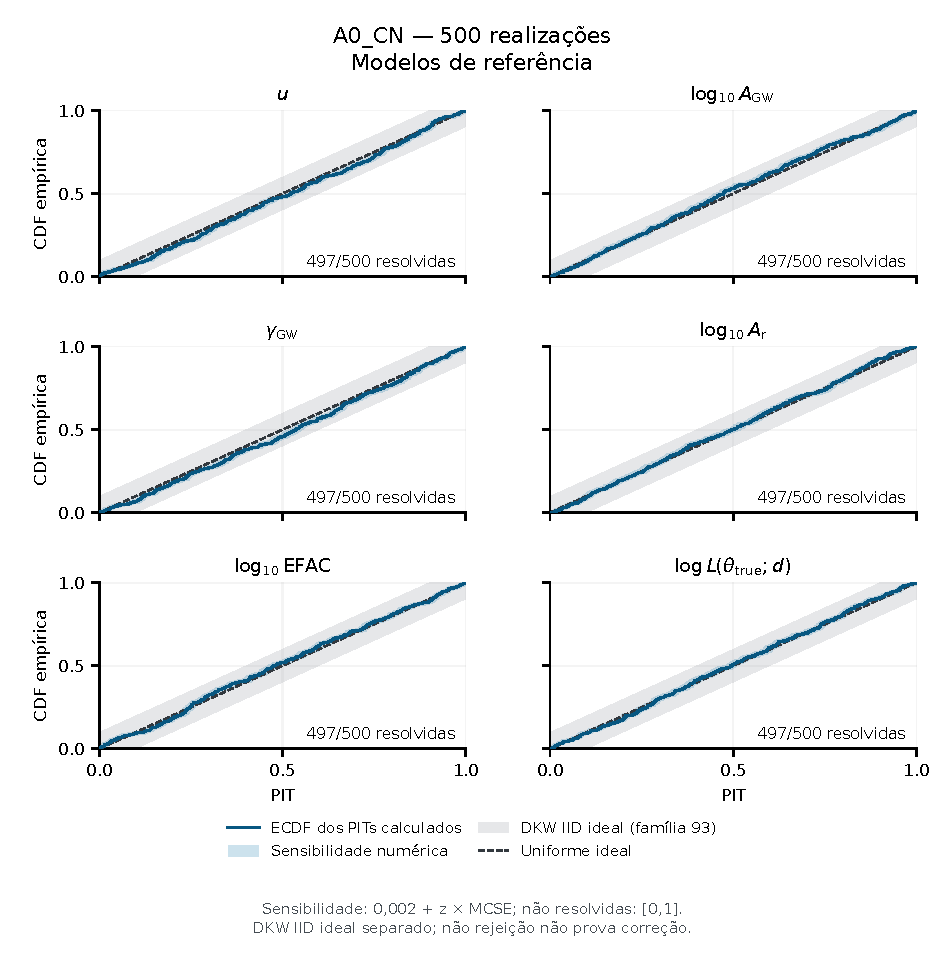
\includegraphics[width=\textwidth]{../figures/C07/synthesis/ecdf_A0_CN.pdf}
 \caption{Calibração de A0\_CN nas 500 realizações da priori. As seis
 funções incluem os cinco parâmetros e a log-verossimilhança na
 verdade. A referência probabilística é a normal complexa própria;
 não há aproximação normal das estatísticas quadráticas neste modelo.}
 \label{fig:c07-sbc-a0}
\end{figure}
\begin{figure}[p]
 \centering
 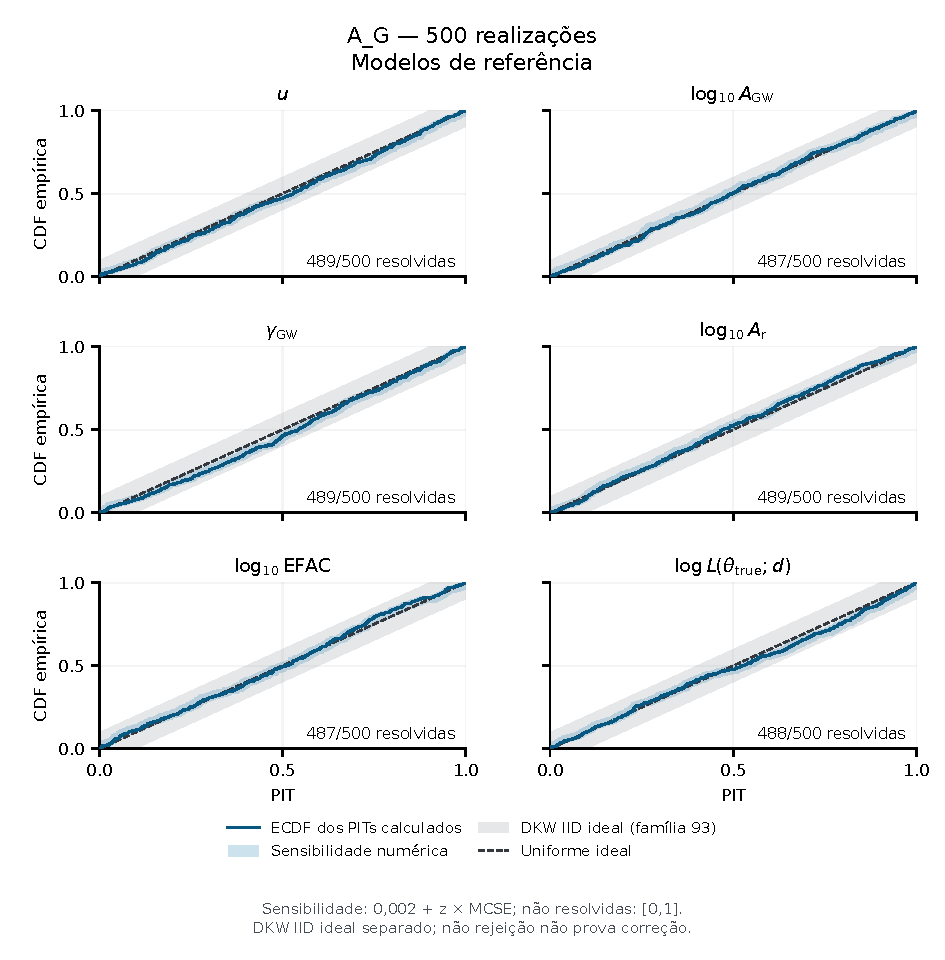
\includegraphics[width=\textwidth]{../figures/C07/synthesis/ecdf_A_G.pdf}
 \caption{Controle A\_G com observações normais de momentos pareados,
 preservando os canais de frequência. As faixas numéricas conservam
 todos os dados, inclusive as funções não resolvidas.}
 \label{fig:c07-sbc-ag}
\end{figure}
\begin{figure}[p]
 \centering
 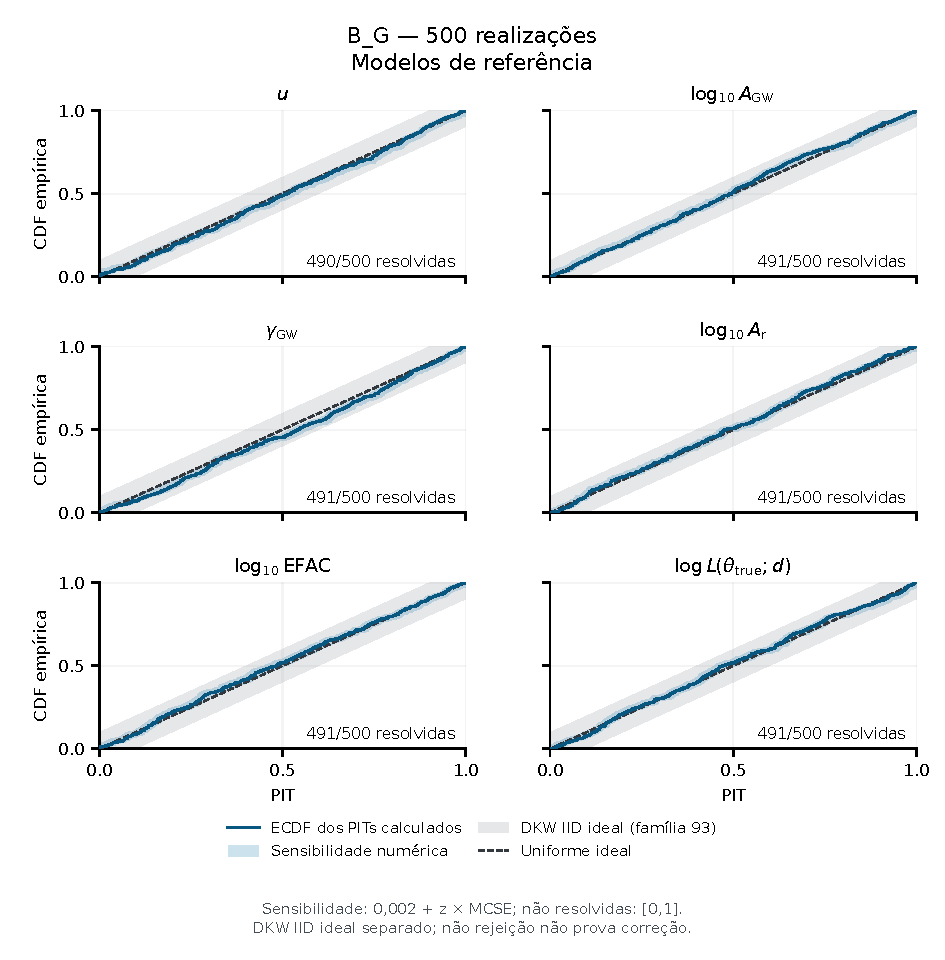
\includegraphics[width=\textwidth]{../figures/C07/synthesis/ecdf_B_G.pdf}
 \caption{Controle B\_G após compressão fixa das observações normais.
 A distribuição normal comprimida é exata para esse controle. A
 compatibilidade com SBC não afirma que a compressão preserve toda
 a informação de A\_G.}
 \label{fig:c07-sbc-bg}
\end{figure}

\subsection{Aproximação normal nas observações físicas}

Na família separada de 62 hipóteses, A\_CN teve oito rejeições
nominais, das quais seis persistiram em toda a sensibilidade numérica.
B\_CN teve cinco rejeições nominais e quatro robustas.
Os desvios robustos concentram-se no fator de ruído branco e na
log-verossimilhança na verdade. Não são treze descobertas
independentes: diferentes testes reutilizam os mesmos PITs e dados.
As Figuras~\ref{fig:c07-sbc-acn} e~\ref{fig:c07-sbc-bcn} mostram
as distribuições empíricas completas.

O contraste é particularmente claro na cobertura central de 90\%
de \(\log_{10}E\): as contagens nominais foram 446/500 em A0\_CN,
313/500 em A\_CN e 412/500 em B\_CN. As frações compatíveis com os
envelopes numéricos de A\_CN e B\_CN foram, respectivamente,
\([0{,}598;0{,}650]\) e \([0{,}802;0{,}838]\). Seus testes binomiais
continuam rejeitando após Holm mesmo no extremo conservador da
sensibilidade. Nos controles correspondentes A\_G e B\_G, as
contagens foram 449/500 e 457/500.

Esses resultados demonstram uma limitação da aproximação normal
neste domínio de simulação, já com a resposta dispersiva correta.
A\_CN preserva as frequências e ainda apresenta o desvio; portanto,
este não pode ser atribuído exclusivamente à perda de frequência.
B\_CN apresenta uma cobertura mais próxima da nominal nesse
parâmetro, sem recuperar a calibração. A soma de contribuições pode
alterar a qualidade da aproximação normal; a campanha, por si só,
não estabelece uma lei universal de melhora com a compressão.

\begin{figure}[p]
 \centering
 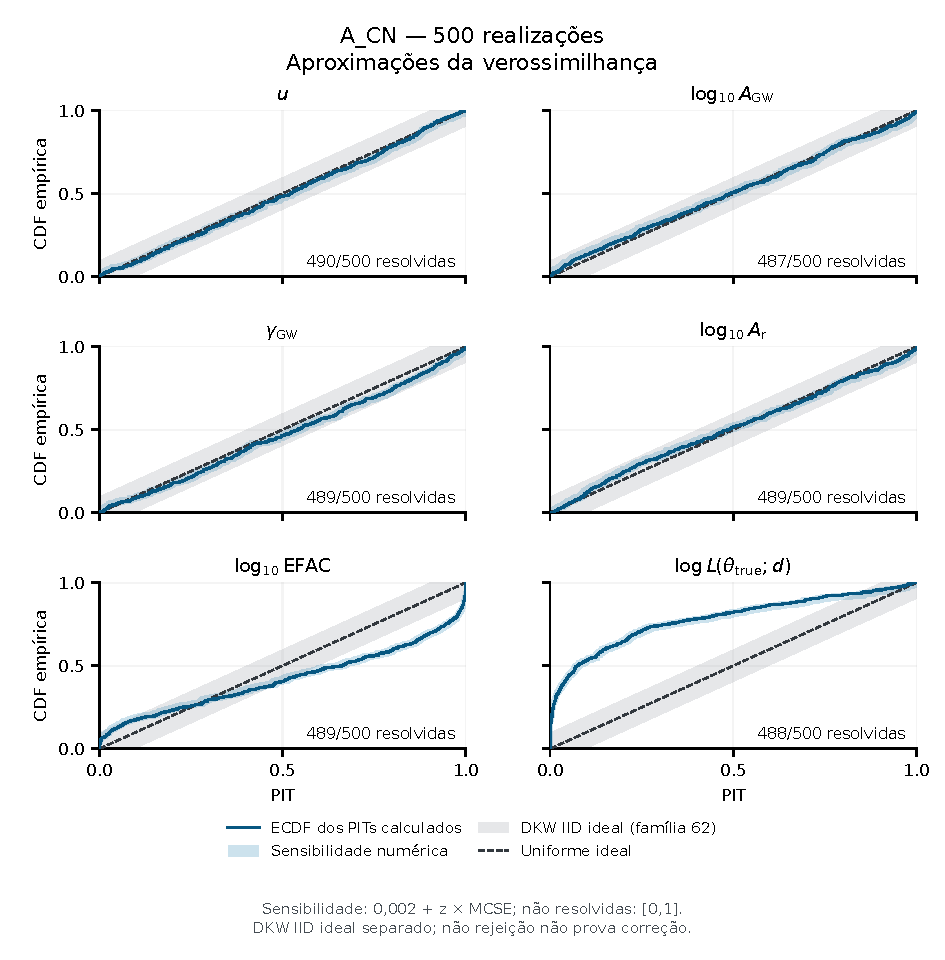
\includegraphics[width=\textwidth]{../figures/C07/synthesis/ecdf_A_CN.pdf}
 \caption{Aproximação A\_CN nas estatísticas quadráticas físicas,
 mantendo a frequência explícita. Os desvios do fator de ruído branco
 e da log-verossimilhança permanecem visíveis após incorporar a
 sensibilidade numérica.}
 \label{fig:c07-sbc-acn}
\end{figure}
\begin{figure}[p]
 \centering
 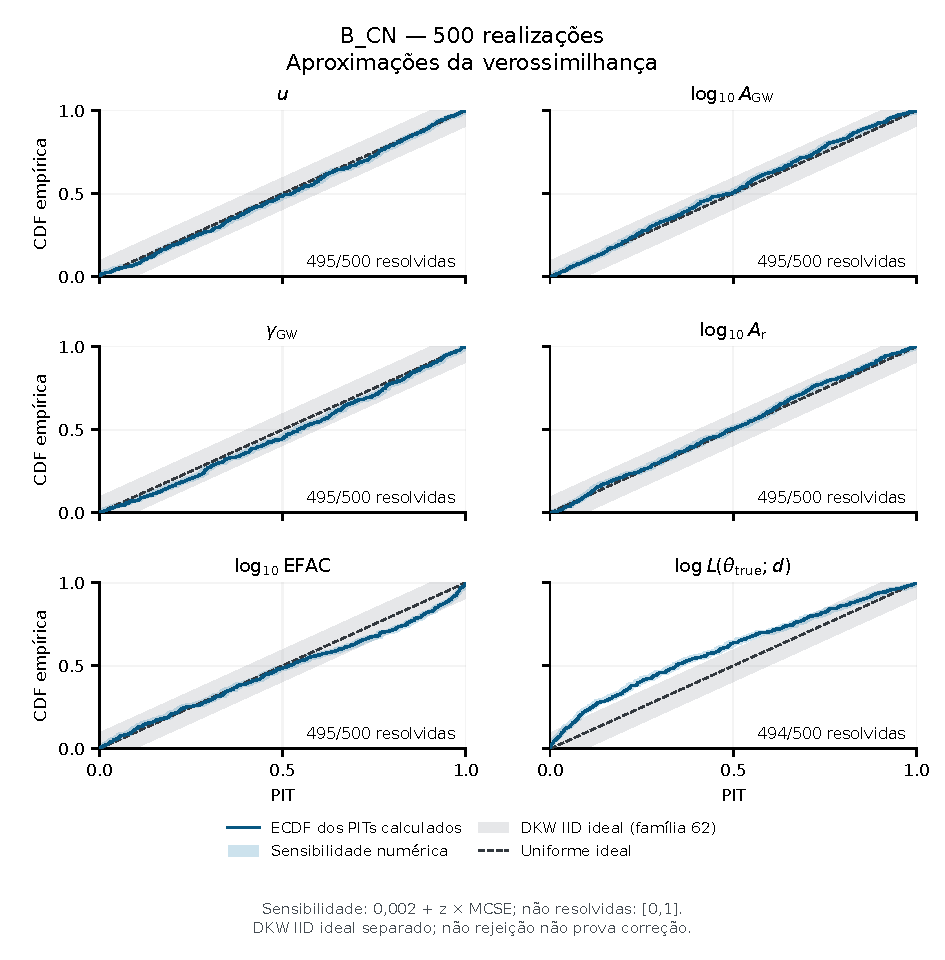
\includegraphics[width=\textwidth]{../figures/C07/synthesis/ecdf_B_CN.pdf}
 \caption{Aproximação B\_CN aplicada às estatísticas físicas
 comprimidas. A redução dos desvios em alguns diagnósticos não
 equivale à recuperação de uma distribuição probabilística exata.}
 \label{fig:c07-sbc-bcn}
\end{figure}

\subsection{Massa, comparações pareadas e limites da conclusão}

Os testes KS marginais da massa adimensional \(u\) não rejeitaram em
nenhum dos cinco modelos. Os valores ajustados de Holm foram 1 e
os valores nominais de \(D_{\rm KS}\) ficaram entre 0,031 e 0,038.
A cobertura central nominal da massa variou de 455/500 a 460/500;
a cobertura do limite superior de 95\%, de 478/500 a 482/500.
A Tabela~\ref{tab:c07-cobertura-massa} apresenta os intervalos
binomiais e as frações possíveis. A calibração marginal da massa
não implica calibração conjunta dos parâmetros, como evidencia o
resultado do ruído branco, nem exclui desvios condicionais em regiões
particulares da priori.

Dos quinze contrastes pareados de cobertura central, oito rejeitaram
nominalmente após Holm; dois permaneceram robustos à sensibilidade.
Ambos envolvem \(\log_{10}E\): A\_CN menos B\_CN apresentou diferença
nominal de \(-0{,}198\), com faixa numérica \([-0{,}240;-0{,}152]\);
A0\_CN menos A\_CN apresentou \(0{,}266\), com faixa
\([0{,}226;0{,}308]\). As faixas numéricas representam ambiguidade
nas contagens observadas, não intervalos de confiança populacionais.
Nenhum contraste da massa foi uma rejeição nominal. Os testes e
intervalos completos, incluindo os retângulos conservadores de
contagens discordantes, permanecem no produto de síntese.

As diferenças de quantis calculadas nas 500 realizações são
exploratórias: sua incerteza horizontal de integração não foi
certificada apenas pela precisão das CDFs. O estudo da compressão
usará uma subamostra fixada por protocolo para reavaliar essas
incertezas. Não se interpreta aqui uma diferença nominal de limites
superiores como viés confirmado da massa, nem uma diferença de
normalizações entre espaços de dados distintos como fator de Bayes.

A campanha fornece uma referência operacional validada e identifica
falhas probabilísticas que devem acompanhar as comparações futuras.
O resultado não é uma restrição observacional à massa do gráviton.
Todas as conclusões se referem à geometria, à priori, aos ruídos e
aos quatro canais do experimento simulado; os controles de valores
fixos abaixo examinam uma pergunta condicional diferente.
\section{Injeções fixas e ausência de sinal}
\label{sec:c07-injecoes-fixas}

A campanha de controle concluiu as 96 inferências A0, com 32 dados
por cenário, sem repetir o sorteio depois dos diagnósticos. Foram
contabilizadas 3146112 avaliações de treino e 31457280 de produção,
num total de 34603392. Os cinco controles agregados passaram nos
96 alvos. Dos 448 PITs aplicáveis, 32 correspondem à identidade
estrutural \(F_u(0)=0\); os outros 416 satisfizeram os critérios
numéricos por função. Os 128 PITs sem verdade definida no cenário
sem sinal foram mascarados e não entraram em coberturas.

% Existing summary only; no new statistical tests.
% SHA256: 1273de6e7f2b835a5c349c5df243b60ac5f865ff0f55f61bfb2715e0ac0c11d5
\begin{table}[htbp]
\centering
\caption{Funções resolvidas nos três cenários fixos: 32 dados A0 em cada cenário.}
\label{tab:c07-fixed-resolucao}
\begingroup\small\setlength{\tabcolsep}{4pt}
\begin{tabular}{@{}lrrrrrr@{}}
\toprule
Cenário & $u$ & $\log A$ & $\gamma$ & $\log A_r$ & $\log E$ & $\log L$ \\
\midrule
$u=0$, com GW & 32$^\ast$ & 32 & 32 & 32 & 32 & 32 \\
$u=0{,}995$, com GW & 32 & 32 & 32 & 32 & 32 & 32 \\
Sem GW & --- & --- & --- & 32 & 32 & --- \\
\bottomrule
\end{tabular}
\endgroup
\par\smallskip\begin{minipage}{0.96\textwidth}\footnotesize O asterisco indica $F_u(0)=0$ estrutural, sem integração numérica. Traços indicam ausência de verdade geradora definida: sem GW não há massa, amplitude ou inclinação do sinal a recuperar. As duas funções de ruído permanecem aplicáveis. Nenhum dado é removido.\end{minipage}
\end{table}
\begin{table}[htbp]
\centering
\caption{Coberturas condicionais selecionadas nos cenários fixos.}
\label{tab:c07-fixed-coberturas}
\begingroup\small\setlength{\tabcolsep}{4pt}
\begin{tabular}{@{}lllr rr@{}}
\toprule
Cenário & Par. & Evento & Cont. & IC 95\% & Faixa \\
\midrule
$u=0$, com GW & $u$ & $F\leq0{,}90$ & 32/32 & $[0{,}891;1]$ & $[1;1]$ \\
$u=0$, com GW & $u$ & $0{,}05\leq F\leq0{,}95$ & 0/32 & $[0;0{,}109]$ & $[0;0]$ \\
$u=0{,}995$, com GW & $u$ & $F\leq0{,}90$ & 0/32 & $[0;0{,}109]$ & $[0;0]$ \\
$u=0{,}995$, com GW & $u$ & $0{,}05\leq F\leq0{,}95$ & 0/32 & $[0;0{,}109]$ & $[0;0]$ \\
Sem GW & $\log A_r$ & $F\leq0{,}90$ & 21/32 & $[0{,}468;0{,}814]$ & $[0{,}625;0{,}688]$ \\
Sem GW & $\log A_r$ & $0{,}05\leq F\leq0{,}95$ & 30/32 & $[0{,}792;0{,}992]$ & $[0{,}938;0{,}938]$ \\
Sem GW & $\log E$ & $F\leq0{,}90$ & 27/32 & $[0{,}672;0{,}947]$ & $[0{,}844;0{,}875]$ \\
Sem GW & $\log E$ & $0{,}05\leq F\leq0{,}95$ & 29/32 & $[0{,}750;0{,}980]$ & $[0{,}875;0{,}906]$ \\
\bottomrule
\end{tabular}
\endgroup
\par\smallskip\begin{minipage}{0.96\textwidth}\footnotesize $F$ é a CDF posterior na verdade. Os ICs de Clopper--Pearson são ponto a ponto, condicionados à contagem calculada; as faixas usam a sensibilidade numérica operacional e $[0,1]$ para funções não resolvidas. Em $u=0$, as coberturas de $[0,U_{90}]$ e do intervalo central são estruturalmente 1 e 0. Não se exige cobertura nominal de 90\% para toda verdade fixa e não se executa SBC nestes cenários.\end{minipage}
\end{table}
\begin{table}[htbp]
\centering
\caption{Quantis de massa calculados: descrição das 32 realizações por cenário.}
\label{tab:c07-fixed-quantis}
\begingroup\small\setlength{\tabcolsep}{4pt}
\begin{tabular}{@{}lrrrr@{}}
\toprule
Cenário & Mediana $Q_{50}$ & Mediana $Q_{90}$ & Mediana $Q_{95}$ & Extremos $Q_{95}$ \\
\midrule
$u=0$, com GW & $0{,}494$ & $0{,}897$ & $0{,}948$ & $[0{,}870;0{,}961]$ \\
$u=0{,}995$, com GW & $0{,}527$ & $0{,}908$ & $0{,}954$ & $[0{,}923;0{,}970]$ \\
Sem GW & $0{,}531$ & $0{,}910$ & $0{,}955$ & $[0{,}950;0{,}959]$ \\
\bottomrule
\end{tabular}
\endgroup
\par\smallskip\begin{minipage}{0.96\textwidth}\footnotesize As medianas e os extremos são tomados entre os 32 dados; não são intervalos de erro numérico. Precisão da CDF não certifica precisão horizontal dos quantis. Sem GW, estes números descrevem o ajuste de um modelo com sinal, sem representar recuperação de uma massa geradora nem detecção.\end{minipage}
\end{table}


Em \(u=0\), a cobertura de \([0,U_{90}]\) é exatamente um, enquanto
um intervalo central de caudas iguais exclui a extremidade zero e
tem cobertura zero. São propriedades do suporte contínuo do modelo,
não resultados de uma falha do integrador. Os intervalos binomiais
mostrados para 32/32 e 0/32 descrevem as contagens; a afirmação
estrutural é mais forte e não depende dessa amostra.

Próximo à borda, em \(u=0{,}995\), nenhum dos 32 intervalos centrais
de 90\% ou limites \([0,U_{90}]\) cobriu a massa verdadeira. Esse
resultado permanece na análise de sensibilidade dos PITs.
Para cada evento, o intervalo binomial pontual de 95\% da cobertura
condicional foi \([0;0{,}109]\). A mediana dos limites calculados
\(Q_{95}\) foi 0,954, e seus extremos entre os dados ficaram em
\([0{,}923;0{,}970]\). Essas descrições de quantis não constituem
certificados de erro horizontal, mas tornam visível a proximidade
com o quantil 0,95 da priori uniforme. A inferência tem capacidade
limitada de deslocar seus limites até essa verdade extrema neste
cenário; não se pode usar a compatibilidade de SBC sob a priori
como garantia de cobertura em toda massa fixa.

Sem sinal gravitacional, a geração usa exatamente covariância de
ruído; a análise ainda ajusta o modelo com sinal. Os quantis de massa
calculados descrevem esse ajuste. Não há massa gravitacional
verdadeira a recuperar, nem amplitude finita do sinal a comparar
com uma priori em logaritmo. A mediana de \(Q_{95}\), 0,955, não
constitui detecção nem limite observado de massa. As coberturas
centrais dos dois parâmetros de ruído foram 30/32 e 29/32, com as
incertezas binomiais da Tabela~\ref{tab:c07-fixed-coberturas}.

\section{Rastreabilidade e alcance da validação}

A síntese preserva as matrizes de PITs, seus envelopes, quantis
calculados, contagens, testes ajustados e identificadores de origem.
Uma implementação independente recalculou 6202 verificações do
resumo, incluindo KS, coberturas, Clopper--Pearson, Holm e os
contrastes pareados. A maior diferença foi
\(1{,}43\times10^{-14}\), no logaritmo de uma probabilidade de
cauda DKW. Separadamente, a leitura dos 2500 diagnósticos compactos
reconstruiu exatamente os 15000 indicadores de resolução por função,
sem chamar o sintetizador original ou ler os arquivos brutos.
As causas de inelegibilidade se sobrepõem: 222 funções falharam na
guarda de pesos, 32 na precisão da CDF, seis na guarda de saturação
e uma na comparação entre réplicas da própria função.

Os produtos da campanha principal foram compactados sem perda;
125233 arquivos preservados foram restaurados em uma pasta nova e
comparados pelos respectivos hashes. O arquivo inclui propostas,
sementes, estados, diagnósticos e recibos de retirada. Os grandes
arrays brutos retirados não são declarados como presentes: sua
reprodução depende das sementes, das fontes e do ambiente numérico
vinculados ao plano. A integridade do arquivo e a aceitação
científica são verificações distintas.

Os resultados satisfazem o objetivo desta etapa de estabelecer uma
referência e delimitar suas falhas. Os modelos correspondentes à
distribuição geradora são compatíveis com SBC no domínio simulado;
as aproximações normais nas estatísticas físicas apresentam desvios
que não desaparecem com a resolução de integração adotada.
Permanecem explícitos os PITs não resolvidos, a precisão horizontal
pendente dos quantis e a cobertura condicional desfavorável perto
da borda. A etapa seguinte compara respostas de frequência de
referência contra esse conjunto, conservando os controles e as
incertezas numéricas.
